\documentclass[11pt]{article}
\usepackage[english]{babel}
\usepackage{natbib}
\usepackage{url}
\usepackage[utf8x]{inputenc}
\usepackage{amsmath}
\usepackage{graphicx}
\graphicspath{{images/}}
\usepackage{parskip}
\usepackage{fancyhdr}
\usepackage{vmargin}
\setcitestyle{square}
\setmarginsrb{3 cm}{2.5 cm}{3 cm}{2.5 cm}{1 cm}{0.75 cm}{1 cm}{1.5 cm}
\usepackage[justification=centering]{caption}
\title{Assignment3 - Advanced Machine Learning}								% Title
										% Date

\makeatletter
\let\thetitle\@title
\let\theauthor\@author
\let\thedate\@date
\makeatother

\pagestyle{fancy}
\fancyhf{}
\rhead{\theauthor}
\lhead{\thetitle}
\cfoot{\thepage}

\begin{document}

%%%%%%%%%%%%%%%%%%%%%%%%%%%%%%%%%%%%%%%%%%%%%%%%%%%%%%%%%%%%%%%%%%%%%%%%%%%%%%%%%%%%%%%%%

% \begin{titlepage}
% 	\centering
%     \vspace*{0.5 cm}
%     \includegraphics[scale = 0.075]{IIT_Delhi_logo.png}\\[1.0 cm]	% University Logo
%     \textsc{\LARGE Indian Institute of Technology Delhi}\\[2.0 cm]	% University Name
% 	\textsc{\LARGE MCL142 Term Paper}\\[0.5 cm]				% Course Code
% 	\rule{\linewidth}{0.2 mm} \\[0.4 cm]
% 	{ \huge \bfseries \thetitle}\\
% 	\rule{\linewidth}{0.2 mm} \\[3.5 cm]
	
% 	\begin{minipage}{0.4\textwidth}
% 		\begin{flushleft} \large
% 			\emph{Submitted To:}\\
% 			Dr. M.R. Ravi\\
% 			Professor\\
% 			Mechanical Engg. Dept.\\
% 			IIT Delhi
% 			\end{flushleft}
% 			\end{minipage}~
% 			\begin{minipage}{0.4\textwidth}
            
% 			\begin{flushright} \large
% 			\emph{Submitted By :} \\
% 			Hritik Bansal\\
% 			(2016EE10071)\\
% 			Gantavya Bhatt\\
% 			(2016EE10694)\\
% 			Anubhav Bhatia\\
% 			(2016EE10835)\\
% 		\end{flushright}
        
% 	\end{minipage}\\[2 cm]
	
% \end{titlepage}
\begin{center}
    \textbf{ELL888 - Assignment 3} \\
\end{center}
{\footnotesize \textbf{Nishad Singhi(2016EE10107), Hritik Bansal(2016EE10071), Gantavya Bhatt(2016EE10694)}}
\section{Problem Statement}

\begin{itemize}
    \item Choose 2 datasets - one gray scale and color each (except for MNIST).
    \item Design a classifier for a classification task on the choosen datasets.
    \item Design a generative model (GAN and it's variants or VAE and it's variants) on both datasets.
    \item Break the classifier by creating atleast 2 types of adversarial attacks on the trained classifiers.
    \item Finally use the trained generative models to make the classifier robust against those attacks.
\end{itemize}

\section{Dataset used}
\begin{flushleft}
The dataset we chose were\textbf{ CIFAR-10 }and \textbf{Kuzushiji MNIST.} 
The CIFAR-10 dataset contains 60,000 32x32 color images in 10 different classes.The 10 different classes represent airplanes, cars, birds, cats, deer, dogs, frogs, horses, ships, and trucks. There are 6,000 images of each class. Whereas, Kuzushiji MNIST is a recent dataset released in December'18 comprising of old Japanese characters of hiragana script. Kuzushiji-MNIST contains 70,000 28x28 grayscale images spanning 10 classes (one from each column of hiragana). 10,000 are used for the cross-validation and testing. CIFAR-10 being a common dataset, we are not showing its image here as an introduction. 
\end{flushleft}
\begin{center}
        \begin{figure}[h]
        \centering
          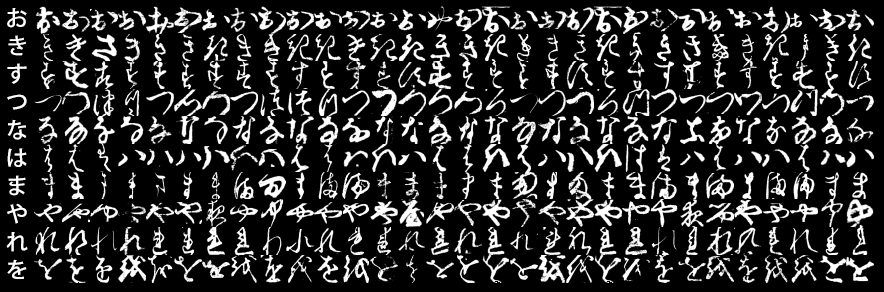
\includegraphics[width=135mm, height=50mm]{kmnist_pic.png}
          \caption{ KMNIST dataset. First column being the true class, the rest being the images in the dataset \cite{ref3}
          }
          \label{fig:Piston}
        \end{figure}
\end{center}

\section{Attacks and Implementation details}
\begin{itemize}
    \item In total we tried three different type of attacks on our 2 classifiers. The first kind of attack being the Fast Gradient Sign method, Projected Gradient Descent attack and Carnili Wagner Attack. 
    \item The FGSM attack is a white box attack in where we have the complete information of our model. We did 2 type of FGSM attacks on our models. The first attack being a non-targetted FGSM and the other one being the targeted FGSM. 
    \item The untargeted FGSM involved doing the gradient ascent on the loss landscape with respect to the input images in the hypercube (for the valid image).
    \item The Targeted FGSM invovled the doing a gradient descent on the loss landscape of the input image and the targeted class. 
    \item The projected Gradient Descent attack was trained for 40 iterations followed by clipping
    \item The Carlini Wagner attack involved the modified optimization problem on the tanh space with L2 as a distance metric. 
\end{itemize}
\begin{center}
        \begin{figure}[h]
        \centering
          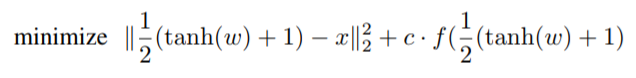
\includegraphics[width=100mm, height=10mm]{CW.PNG}
        \end{figure}
\end{center}
\[f(x') = max(max(Z(x'_i), i\neq t ) -  Z(x'_t), -\kappa ) \]
\emph{Z is the pre-activation of the ultimate layer}
\section{Classifier results}
\begin{table}[!h]
\centering
\begin{tabular}{c|c}
$Datasets$& Accuracy  \\\hline
CIFAR-10 & 79.88 \% \\
Kuzushiji-MNIST	& 94.18 \% 
\end{tabular}
\caption{\label{Table 1: } Our Classifier on non-adverserial examples}
\end{table}
These are our classifier accuracies for the CIFAR-10 and the Kuzushiji MNIST dataset.
\section{Adverserial Attacks}
In this section, we will discuss the outputs of different attack algorithms and their impact on the accuracy of our models. Firstly, we will discuss the image mis-classified by KMNIST and the CIFAR-10 classifier inspite of being so close. 
\begin{center}
        \begin{figure}[h]
        \centering
          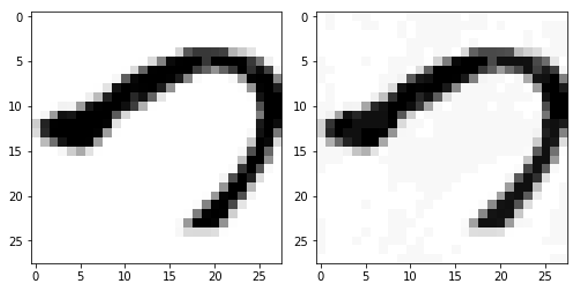
\includegraphics[width=60mm, height=40mm]{attack_FGSM_unt_kuzu.png}
          \caption{ Image misclassified as hiragana character "ya" instead of "shi" (a) Non adverserial image, (b) Adverserial.
          }
          \label{fig:Piston}
        \end{figure}
\end{center}

\begin{center}
        \begin{figure}[!h]
        \centering
          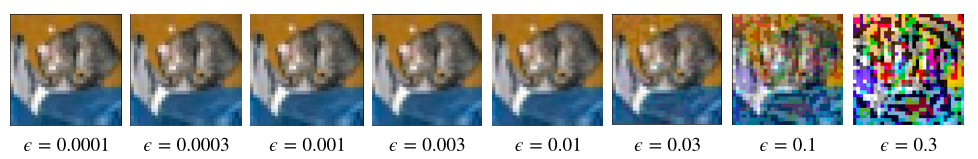
\includegraphics[width=150mm, height=30mm]{adverserial_examples_CIFAR_FGSM.png}
          \caption{ Image after the perturbation by the FGSM attacks on CIFAR-10
          }
          
          \label{fig:Piston}
        \end{figure}
\end{center}
\subsection{Impact on accuracy of classifier by increasing attack power}  

As it can be clearly seen, as the value of the epsilon increases, the misclassification rate increases. We kept the epsilon in such a way that the image remains in the valid dimensions, that is the pixels value of the image remain in the 0 to 1 hypercube. 

\begin{center}
        \begin{figure}[!h]
        \centering
          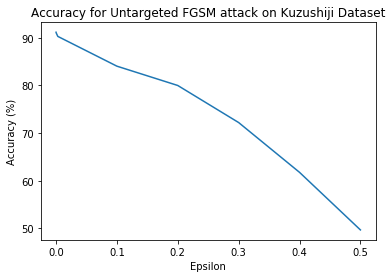
\includegraphics[width=70mm, height=40mm]{kuzu_untargeted_FGSM_accuracy.png}
          \caption{ Accuracy versus epsilon in untargetted attack FGSM on Kuzushiji
          }
          \label{fig:Piston}
        \end{figure}
\end{center}

\begin{center}
        \begin{figure}[!h]
        \centering
          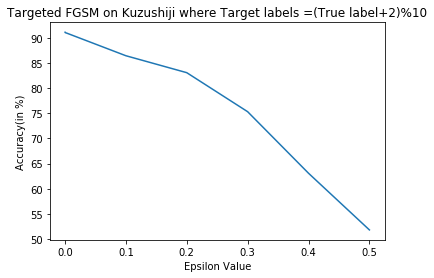
\includegraphics[width=80mm, height=50mm]{kuzushiji_targetedfgsm.png}
          \caption{ Accuracy versus epsilon in targeted attack FGSM on Kuzushiji
          }
          \label{fig:Piston}
        \end{figure}
\end{center}


\begin{center}
        \begin{figure}[h]
        \centering
          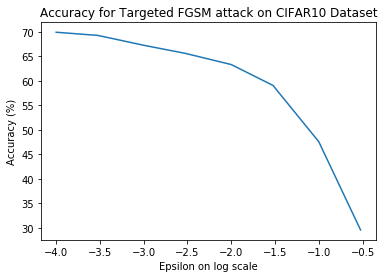
\includegraphics[width=80mm, height=50mm]{cifar targeted fgsm accuracy.png}
          \caption{ Accuracy versus epsilon in untargetted attack FGSM on CIFAR-10
          }
          \label{fig:Piston}
        \end{figure}
\end{center}

\begin{center}
        \begin{figure}[!h]
        \centering
          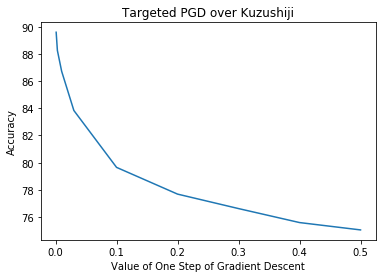
\includegraphics[width=80mm, height=50mm]{kuzushiji_targetedpgd.png}
          \caption{ Accuracy versus epsilon for PGD attack
          }
          \label{fig:Piston}
        \end{figure}
\end{center}
\pagebreak

\begin{center}
        \begin{figure}[!h]
        \centering
          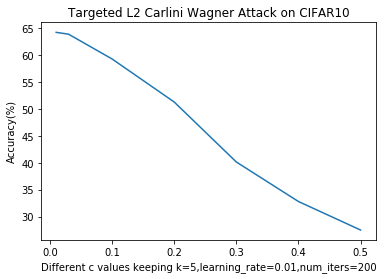
\includegraphics[width=80mm, height=50mm]{CIFAR10_CW.png}
          \caption{ Targeted L2 CW attack on CIFAR10
          }
          \label{fig:Piston}
        \end{figure}
\end{center}

\begin{center}
        \begin{figure}[!h]
        \centering
          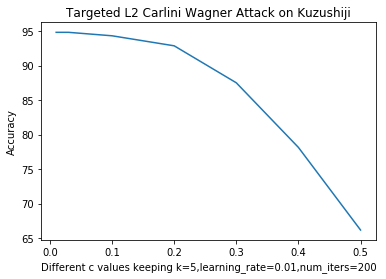
\includegraphics[width=80mm, height=50mm]{CW_kuzu_C_value.png}
          \caption{ Targeted L2 CW attack on Kuzushiji with varying C
          }
          \label{fig:Piston}
        \end{figure}
\end{center}

\begin{center}
        \begin{figure}[!h]
        \centering
          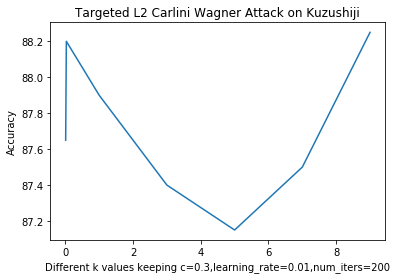
\includegraphics[width=80mm, height=50mm]{CW_kuzu_K_values.png}
          \caption{ Targeted L2 CW attack on Kuzushiji with varying K
          }
          \label{fig:Piston}
        \end{figure}
\end{center}

\emph{As a strange observation, it was observed that while varying the K (the confidence in CW attack), the accuracy showed a strange behavior of not decreasing continuously to low values. Also, the variation was insignificatn (2\%). Thus, we can say that the CW attack didn't depend much on the K values on which we did our experimentation.}

\section{Protection against the Dark Arts}
\subsection{Training on Adverserial Images}
At first, we tried training on the Adverserial Images to make the classifier robust against the adverserial examples.Training the classifier on the adverserial example acts as a regularizer as well as a data augmentation. 
\begin{table}[!h]
\centering
\begin{tabular}{c|c|c}
$Datasets$& Accuracy after attack & Accuracy after training on Adv. Example  \\\hline
Kuzushiji-MNIST	& 94.18 \%  & 92.15\%\\
CIFAR-10 & 79.88 & 77.67\% 

\end{tabular}
\caption{\label{Table 1: }Improved Accuracy on adverserial attacks after training on adverserial examples}
\end{table}
\\

Thus we saw that training on the adverserial examples can give appealing results at the test time. However, there can be a lot more adverserial example and even some of them lying on the data manifold. Thus, as a generalization, this might not be robust against the examples on the data manifold. 
\subsection{Generative Models}
We also used the Generative Models to get rid of the adverserial examples also for the data augmentation. The Generative model we trained was VAE and CNN-VAE. 

\subsubsection{Generation of Images}
With the help of VAE, we generated the following images. These images were close to the image in the data distribution and had low reconstruction errors.

\begin{center}
        \begin{figure}[!h]
        \centering
          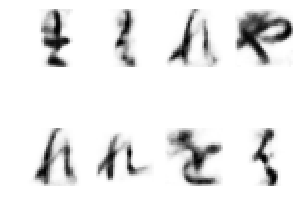
\includegraphics[width=80mm, height=60mm]{1.png}
          \caption{ VAE Generated Images
          }
          \label{fig:Piston}
        \end{figure}
\end{center}
\begin{center}
        \begin{figure}[!h]
        \centering
          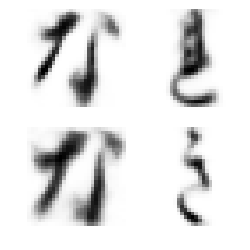
\includegraphics[width=50mm, height=40mm]{2.png}
          \caption{ VAE Generated Images
          }
          \label{fig:Piston}
        \end{figure}
\end{center}

\begin{center}
        \begin{figure}[!h]
        \centering
          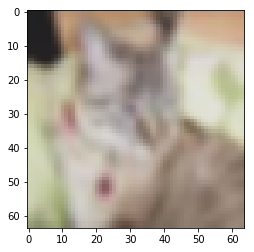
\includegraphics[width=60mm, height=40mm]{vae_cifar10_1.png}
          \caption{ VAE Generated Images
          }
          \label{fig:Piston}
        \end{figure}
\end{center}
\emph{It was seen that when we passed the adverserial examples from the encoder the latent space representation of the adverserial example was far from the original image. Thus, the reconstructed image was far from what was in the adverserial example.} \\
\emph{This problem can be solved by imposing the Lipschitz condition while training the classifier so that in the latent space the adverserial image will be close to the true image. Hence, we can get a better reconstruction of the image from the decoder.}\\
\pagebreak
\begin{table}[!h]
\centering
\begin{tabular}{c|c|c}
$Attack$& Accuracy after passing through VAE & Accuracy on reconstructed true input\\\hline
CW attack	& 27.18\% & 82.15\% \\
FGSM & 33.11\%  & 82.15\% \\
PGD & 30.12\%  & 82.15\% 
\end{tabular}
\caption{\label{Table 1: } Results using latent variable of adverserial examples to reconstruct on KMNIST }
\end{table}
\\

Inspired from Defense GAN, where we solve an optimization problem on the z space\cite{ref5}, we tried to do 1 Nearest Neighbour for 10000 images generated by the Decoder of the VAE. The nearest images after the KNN is the closest image in the data manifold to the adverserial example.\\
\emph{The KNN is much faster as compared to solving an optimization problem. Thus, we think that on the execution time, if we take less noise instances then this can be done in the real time.}

\begin{table}[!h]
\centering
\begin{tabular}{c|c|c}
$Attack$& Accuracy after attack & Accuracy after KNN on VAE output\\\hline
CW attack	& 25.18\% & 48.15\% \\
FGSM & 34.11\%  & 59.75\% \\
PGD & 32.12\%  & 54.15\% 
\end{tabular}
\caption{\label{Table 1: }Results on KMNIST after KNN on VAE outputs}
\end{table}
\\

\begin{table}[!h]
\centering
\begin{tabular}{c|c|c}
$Attack$& Accuracy after attack & Accuracy after KNN on VAE output\\\hline
CW attack	& 29.18\% & 41.15\% \\
FGSM & 36.11\%  & 52.75\% \\
PGD & 34.12\%  & 46.15\% 
\end{tabular}
\caption{\label{Table 1: }Results on CIFAR-10 after KNN on VAE outputs}
\end{table}
\\

\section{Conclusions}

\begin{itemize}
    \item A wide variety of attacks like FGSM,PGD and Carlini Wagner were explored in this assignment.
    \item The graphical results of attacks along with their respective parameters were presented above. 
    \item We observed that Carlini Wagner attack reduced our accuracy on both datasets--Kuzushiji and CIFAR10, to a greater extent than when compared to other attacks. This is in agreement with the results of [1], where CW attack was shown to be much better than others. 
    \item Variational Autoencoder was used as a generative model in this assignment due to its well-behaved training procedure.The model produced realistic-loos king images, which can be seen in the figures in the previous sections.
    \item Some methods of defense against these attacks were extensively worked upon this assignment. Substantial improvements were observed in the experiments. 
    \item Our model did not use gradient methods as is done in Defese-GAN. Instead, our approach incorporates k-Nearest Neighbours which is \textbf{computationally less expensive and improves the accuracy substantially}.
\end{itemize}

\begin{thebibliography}{9}

\bibitem{ref1}
Towards Evaluating the robustness of Neural Networks
\\\texttt{https://arxiv.org/abs/1608.04644}
\bibitem{ref2}
Deep Learning for Classical Japanese Literature \\
\texttt{https://arxiv.org/abs/1812.01718}
\bibitem{ref3}
Towards Evaluating the Robustness of Neural Networks
\\\texttt{https://arxiv.org/abs/1608.04644}
\bibitem{ref4}
Defense-GAN: Protecting Classifiers Against Adversarial Attacks Using Generative Models\\
\texttt{https://arxiv.org/abs/1805.06605}
\bibitem{ref5}
Auto-Encoding Variational Bayes\\
\texttt{https://arxiv.org/abs/1312.6114}
\bibitem{ref6}
CIFAR-10 Dataset\\
\texttt{http://academictorrents.com/details/463ba7ec7f37ed414c12fbb71ebf6431eada2d7a}

\end{thebibliography}



\end{document}